\section{Лекция 2. Методы интегрирования дифференциальных уравнений}
\noeqref{eq:l2_sep_var, eq:l2_sep_diff, eq:l2_lipschitz, eq:l2_lagrange}

\begin{flushright}
    14.09.26
\end{flushright}

\subsection{Дифференциальные уравнения с разделяющимися переменными}

\begin{definition}
    Дифференциальным уравнением \textdef{с разделяющимися переменными}
    называется уравнение 1-го порядка вида:
    \begin{equation} \label{eq:l2_sep_var}
        y' = P(x) \cdot Q(y), \tag{1}
    \end{equation}
    где $P \in C(I_x)$ и $Q \in C(I_y)$ — функции, непрерывные на
    соответствующих интервалах $I_x, I_y \subset \R$.
\end{definition}

При анализе и решении уравнения \eqref{eq:l2_sep_var} рассматриваются два
взаимоисключающих случая:
\begin{enumerate}
    \item \textbf{Стационарные корни.} Если существует такое число
    $y_0 \in I_y$, что $Q(y_0) = 0$, то постоянная функция $y(x) \equiv y_0$
    является решением уравнения \eqref{eq:l2_sep_var}. В самом деле, при
    подстановке в левую и правую части получаем верное тождество:
    $0 = P(x) \cdot 0$.
    \item \textbf{Общий случай ($Q(y) \neq 0$).} На интервалах, где
    $Q(y) \neq 0$, разделим обе части уравнения на $Q(y)$ и проинтегрируем по
    независимой переменной $x$:
    \[
        \frac{y'(x)}{Q(y(x))} = P(x) \implies
        \int \frac{y'(x) \, dx}{Q(y(x))} = \int P(x) \, dx
        \iff \int \frac{dy}{Q(y)} = \int P(x) \, dx.
    \]
\end{enumerate}

\textbf{Запись через дифференциалы:}
Представляя производную как отношение дифференциалов $y' = \frac{dy}{dx}$,
уравнение \eqref{eq:l2_sep_var} можно формально записать с разделёнными
переменными:
\begin{equation} \label{eq:l2_sep_diff}
    \frac{dy}{dx} = P(x) \cdot Q(y) \implies \frac{dy}{Q(y)} = P(x) \, dx.
    \tag{2}
\end{equation}

В результате взятия неопределённых интегралов решение может быть получено либо
в \textdef{явном виде} $y = \phi(x, C)$, либо в \textdef{неявном виде}
$\psi(x, y, C) = 0$ (такое соотношение называют \textdef{общим интегралом}
уравнения). К найденному семейству необходимо присоединить постоянные решения
$y = y_0$ (корни уравнения $Q(y) = 0$), если они не входят в общую формулу ни
при каком значении константы $C$.

\begin{example}
    Решить дифференциальное уравнение $y' = x^2 y^3$.

    \begin{proof}[Решение]~\\
        \begin{quote}
            Здесь $P(x) = x^2 \in C(\R)$ и $Q(y) = y^3 \in C(\R)$.
            Приравнивая $Q(y) = 0$, находим стационарное решение $y(x) \equiv 0$.

            Предположим теперь, что $y \neq 0$. Разделим переменные и
            проинтегрируем обе части:
            \[
                \frac{dy}{y^3} = x^2 \, dx \implies
                \int y^{-3} \, dy = \int x^2 \, dx.
            \]
            Вычисляя интегралы, получаем:
            \[
                -\frac{1}{2y^2} = \frac{x^3}{3} + C_0 \quad \Big| \cdot (-2)
                \implies \frac{1}{y^2} = -\frac{2}{3} x^3 + C,
            \]
            где $C = -2C_0 \in \R$ — произвольная постоянная. Выражая $y$,
            находим:
            \[
                y^2 = \frac{1}{C - \frac{2}{3} x^3} \implies
                y(x) = \pm \frac{1}{\sqrt{C - \frac{2}{3} x^3}}.
            \]
            Заметим, что решение $y \equiv 0$ не получается из данной формулы
            ни при каком конечном $C \in \R$ (оно соответствует предельному
            переходу $C \to \infty$), поэтому его необходимо записать в ответ
            отдельно.

            \textbf{Ответ:} $y = \pm \dfrac{1}{\sqrt{C - \frac{2}{3} x^3}}$, а
            также $y = 0$.
        \end{quote}
    \end{proof}
\end{example}

\begin{example}
    Решить дифференциальное уравнение $y' = -\dfrac{x}{y}$.

    \begin{proof}[Решение]~\\
        \begin{quote}
            Здесь $P(x) = -x \in C(\R)$, а $Q(y) = \frac{1}{y} \in C(\R \setminus \{0\})$.
            Значение $y = 0$ не является решением, так как правая часть
            уравнения при $y = 0$ не определена.

            Умножая обе части на $y$ и интегрируя, получаем:
            \[
                y \, dy = -x \, dx \implies \int y \, dy = -\int x \, dx,
            \]
            \[
                \frac{y^2}{2} = -\frac{x^2}{2} + C_0 \implies
                x^2 + y^2 = C, \quad C = 2C_0 > 0.
            \]
            Общий интеграл задаёт семейство концентрических окружностей с
            центром в начале координат. С точки зрения определения решения как
            дифференцируемой функции $y = y(x)$, каждая окружность
            $x^2 + y^2 = R^2$ распадается на две гладкие ветви (верхнюю и
            нижнюю полуокружности):
            \[
                y(x) = \pm \sqrt{R^2 - x^2}, \quad x \in (-R, R).
            \]
            В точках $(\pm R, 0)$ пересечения с осью $Ox$ касательные к
            интегральным кривым становятся вертикальными, а производная
            $y'_x \to \infty$.

            \textbf{Ответ:} $x^2 + y^2 = C$ ($C > 0$, $y \neq 0$).
        \end{quote}
    \end{proof}
\end{example}

\begin{figure}[H]
    \centering
    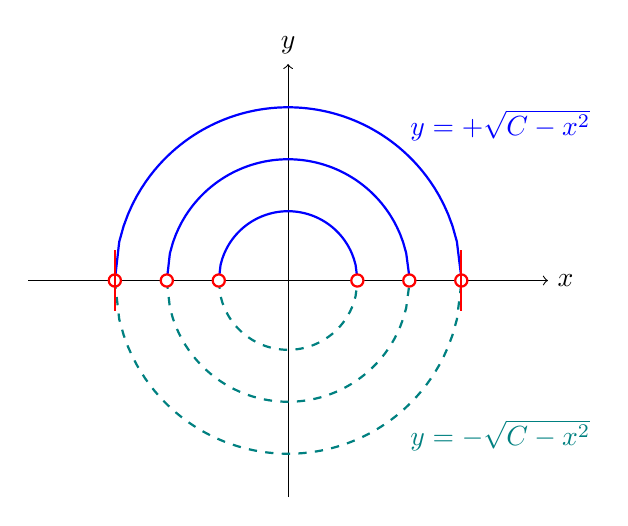
\begin{tikzpicture}[scale=1.1]
        % Оси координат
        \draw[->] (-3, 0) -- (3, 0) node[right] {$x$};
        \draw[->] (0, -2.5) -- (0, 2.5) node[above] {$y$};

        % Семейство полуокружностей
        \foreach \r in {0.8, 1.4, 2.0} {
            \draw[blue, thick, domain=-\r:\r, samples=80]
                plot (\x, {sqrt(\r*\r - \x*\x)});
            \draw[teal, thick, dashed, domain=-\r:\r, samples=80]
                plot (\x, {-sqrt(\r*\r - \x*\x)});
            % Выколотые точки на оси Ox (вертикальные касательные)
            \draw[red, fill=white, thick] (\r, 0) circle (2pt);
            \draw[red, fill=white, thick] (-\r, 0) circle (2pt);
        }

        % Вертикальные штрихи касательных на оси Ox
        \draw[red, thick] (2, -0.35) -- (2, 0.35);
        \draw[red, thick] (-2, -0.35) -- (-2, 0.35);
        \node[above right, blue] at (1.3, 1.5) {$y = +\sqrt{C - x^2}$};
        \node[below right, teal] at (1.3, -1.5) {$y = -\sqrt{C - x^2}$};
    \end{tikzpicture}
    \caption{Интегральные кривые уравнения $y' = -x/y$: верхние и нижние
    полуокружности с выколотыми точками вертикальных касательных при $y = 0$.}
\end{figure}

\subsection{Особые решения задачи Коши}

Рассмотрим задачу Коши для уравнения $y' = f(x, y)$ с начальным условием
$y(x_0) = y_0$.

\begin{definition}
    Решение $y = \phi(x)$ называется \textdef{особым решением}
    дифференциального уравнения, если в каждой точке его графика нарушается
    единственность решения задачи Коши — то есть через каждую его точку
    проходит хотя бы ещё одна интегральная кривая, не совпадающая с $\phi(x)$
    ни в какой сколь угодно малой окрестности этой точки.
\end{definition}

Геометрически особое решение представляет собой \textdef{огибающую} семейства
интегральных кривых: в каждой своей точке огибающая касается некоторой кривой
из общего семейства и имеет с ней общую касательную.

\begin{figure}[H]
    \centering
    \begin{tikzpicture}[scale=1.4]
        % Оси координат
        \draw[->] (-2.8, 0) -- (2.8, 0) node[right] {$x$};
        \draw[->] (0, -1.3) -- (0, 1.3) node[above] {$y$};

        % Особое решение (горизонтальная прямая y = 0)
        \draw[red, very thick] (-2.6, 0) -- (2.5, 0)
            node[above left, red] {$y = \phi(x) = 0$ (особое решение)};

        % Семейство касающихся кубических парабол
        \foreach \c in {-1.5, 0, 1.5} {
            \draw[blue, thick, domain=\c-0.65:\c+0.65, samples=50]
                plot (\x, {2.5 * (\x-\c) * (\x-\c) * (\x-\c)});
            \fill[black] (\c, 0) circle (1.5pt);
            \node[inner sep=1pt] at (\c-0.25, 0) {$($};
            \node[inner sep=1pt] at (\c+0.25, 0) {$)$};
        }

        % Подписи
        \node[blue] at (1.5, -0.95) {частные решения семейства};
    \end{tikzpicture}
    \caption{Особое решение $y = 0$ как огибающая семейства интегральных
    кривых (с выделенными окрестностями точек касания).}
\end{figure}

\subsection{Условие Липшица и теорема Лагранжа}

Для того чтобы сформулировать строгий математический критерий, исключающий
появление особых решений и гарантирующий единственность решения задачи Коши,
введём понятие условия Липшица.

\begin{definition}
    Функция $f(x)$ удовлетворяет \textdef{условию Липшица} на отрезке
    $[a, b] \subset \R$, если существует такая постоянная $L > 0$, что для
    любых двух точек $x_1, x_2 \in [a, b]$ выполняется неравенство:
    \begin{equation} \label{eq:l2_lipschitz}
        \abs{f(x_1) - f(x_2)} \le L \abs{x_1 - x_2}. \tag{3}
    \end{equation}
    Число $L$ называется \textdef{константой Липшица}.
\end{definition}

Геометрически условие Липшица \eqref{eq:l2_lipschitz} означает, что угловой
коэффициент любой хорды (секущей), соединяющей две точки графика функции
$f(x)$ на отрезке $[a, b]$, ограничен по модулю константой $L$:
\[
    \abs{\frac{f(x_1) - f(x_2)}{x_1 - x_2}} \le L.
\]

\begin{theorem}[\textbf{Теорема Лагранжа о конечных приращениях}]
    Пусть функция $f(x)$ непрерывна на отрезке $[a, b]$ и дифференцируема на
    интервале $(a, b)$, то есть $f \in C([a, b]) \cap C^1((a, b))$. Тогда
    существует хотя бы одна внутренняя точка $c \in (a, b)$ такая, что:
    \begin{equation} \label{eq:l2_lagrange}
        f(b) - f(a) = f'(c)(b - a) \iff \frac{f(b) - f(a)}{b - a} = f'(c).
        \tag{4}
    \end{equation}
\end{theorem}

\begin{figure}[H]
    \centering
    \begin{tikzpicture}[scale=1.4]
        % Оси координат
        \draw[->] (-0.3, 0) -- (4.2, 0) node[right] {$x$};
        \draw[->] (0, -0.3) -- (0, 3.4) node[above] {$y$};

        % Координаты концов отрезка
        \def\a{0.8}
        \def\b{3.2}
        \def\fa{1.0}
        \def\fb{2.44}

        % Пунктирные проекции на оси
        \draw[dashed, gray] (\a, 0) node[below, black] {$a$} -- (\a, \fa);
        \draw[dashed, gray] (\b, 0) node[below, black] {$b$} -- (\b, \fb);
        \draw[dashed, gray] (0, \fa) node[left, black] {$f(a)$} -- (\a, \fa);
        \draw[dashed, gray] (0, \fb) node[left, black] {$f(b)$} -- (\b, \fb);

        % Треугольник приращений и секущая
        \draw[dashed] (\a, \fa) -- (\b, \fa);
        \draw[teal, thick] (\a, \fa) -- (\b, \fb);

        % Кривая функции y = f(x)
        \draw[blue, very thick, domain=\a:\b, samples=60]
            plot (\x, {1.0 + 0.6*(\x - \a) + 0.45*sin(180*(\x - \a)/(\b - \a))});

        % Точка c и параллельная касательная
        \def\c{2.0}
        \def\fc{2.17}
        \draw[dashed, red] (\c, 0) node[below] {$c$} -- (\c, \fc);
        \draw[red, thick] (\c - 0.85, \fc - 0.51) -- (\c + 0.85, \fc + 0.51)
            node[above right] {касательная $f'(c)$};

        % Угол наклона секущей
        \draw (\a + 0.55, \fa) arc (0:31:0.55);
        \node at (\a + 0.78, \fa + 0.2) {$\alpha$};

        % Точки
        \fill[blue] (\a, \fa) circle (1.5pt);
        \fill[blue] (\b, \fb) circle (1.5pt);
        \fill[red] (\c, \fc) circle (1.5pt);
    \end{tikzpicture}
    \caption{Геометрический смысл теоремы Лагранжа: касательная в точке
    $c \in (a, b)$ параллельна секущей, проходящей через концы дуги.}
\end{figure}

\begin{proposition}
    Если функция $f(x)$ непрерывно дифференцируема на отрезке $[a, b]$
    ($f \in C^1([a, b])$) или имеет ограниченную производную на $(a, b)$, то
    она удовлетворяет условию Липшица на $[a, b]$.
\end{proposition}

\begin{proof}[Доказательство]~\\
    \begin{quote}
        Возьмём произвольные точки $x_1, x_2 \in [a, b]$ (пусть $x_1 < x_2$).
        По теореме Лагранжа на отрезке $[x_1, x_2]$ найдётся точка
        $c \in (x_1, x_2)$, для которой выполняется равенство
        \eqref{eq:l2_lagrange}:
        \[
            f(x_2) - f(x_1) = f'(c)(x_2 - x_1).
        \]
        Переходя к модулям, оценим правую часть через супремум модуля
        производной на всём отрезке $[a, b]$:
        \[
            \abs{f(x_2) - f(x_1)} = \abs{f'(c)} \cdot \abs{x_2 - x_1} \le
            \sup_{x \in [a, b]} \abs{f'(x)} \cdot \abs{x_2 - x_1}.
        \]
        Полагая $L = \sup_{x \in [a, b]} \abs{f'(x)} < \infty$, получаем
        требуемое неравенство Липшица $\abs{f(x_2) - f(x_1)} \le L \abs{x_2 - x_1}$.
    \end{quote}
\end{proof}

\begin{example}
    Приведём пример функции, которая непрерывна на луче $[0, +\infty)$, но не
    дифференцируема в точке $x = 0$ и \textbf{не удовлетворяет условию
    Липшица} ни на каком отрезке $[0, b]$:
    \[
        f(x) =
        \begin{cases}
            x \ln x, & x > 0, \\
            0, & x = 0.
        \end{cases}
    \]

    \begin{proof}[Исследование функции]~\\
        \begin{quote}
            \textbf{1. Непрерывность на $[0, +\infty)$.}\\
            При $x > 0$ функция непрерывна как произведение элементарных
            функций. Проверим непрерывность справа в точке $x = 0$, вычислив
            предел по правилу Лопиталя:
            \[
                \lim_{x \to +0} (x \ln x) =
                \lim_{x \to +0} \frac{\ln x}{1 / x} =
                \left[ \frac{-\infty}{+\infty} \right] =
                \lim_{x \to +0} \frac{1 / x}{-1 / x^2} =
                -\lim_{x \to +0} x = 0 = f(0).
            \]
            Следовательно, $f \in C([0, +\infty))$.

            \textbf{2. Нарушение условия Липшица в окрестности нуля.}\\
            Предположим от противного, что функция удовлетворяет условию
            Липшица на $[0, b]$ с некоторой константой $L > 0$. Тогда для
            точек $x_1 = 0$ и $x_2 = x \in (0, b]$ должно выполняться:
            \[
                \abs{f(x) - f(0)} \le L \abs{x - 0} \implies
                \abs{x \ln x} \le L x \implies \abs{\ln x} \le L.
            \]
            Однако при $x \to +0$ величина $\abs{\ln x} \to +\infty$ и
            превышает любое наперёд заданное число $L$. Полученное
            противоречие доказывает, что $f(x)$ не удовлетворяет условию
            Липшица вблизи нуля (геометрически это объясняется тем, что
            производная $f'(x) = \ln x + 1 \to -\infty$ при $x \to +0$, и
            график имеет в начале координат вертикальную полукасательную).
        \end{quote}
    \end{proof}
\end{example}

\begin{figure}[H]
    \centering
    \begin{tikzpicture}[scale=1.4]
        % Оси координат
        \draw[->] (-0.4, 0) -- (3.2, 0) node[right] {$x$};
        \draw[->] (0, -0.8) -- (0, 1.5) node[above] {$y$};

        % График f(x) = x ln(x)
        \draw[blue, very thick, domain=0.005:2.4, samples=120]
            plot (\x, {\x * ln(\x)}) node[above left] {$f(x) = x \ln x$};

        % Вертикальная полукасательная в (0,0)
        \draw[red, very thick, -stealth] (0, 0) -- (0, -0.75)
            node[left] {$f'(+0) = -\infty$};
        \fill[red] (0, 0) circle (1.5pt);

        % Точка экстремума x = 1/e
        \draw[dashed, gray] (0.368, 0) node[above] {$\frac{1}{e}$}
            -- (0.368, -0.368);
        \fill[blue] (0.368, -0.368) circle (1.5pt);
        \fill[blue] (1, 0) circle (1.5pt) node[below right] {$1$};
    \end{tikzpicture}
    \caption{График функции $f(x) = x \ln x$: в точке $(0, 0)$ касательная
    становится вертикальной, поэтому наклон секущих неограничен и условие
    Липшица нарушается.}
\end{figure}